\documentclass{article}
\usepackage{graphicx} % Required for inserting images
\usepackage[polish]{babel}
\usepackage[T1]{fontenc}
\usepackage{amsmath}
\usepackage{minted}
\graphicspath{{./images/}}

\title{Algorytmy macierzowe - Drugi zestaw zadań}
\author{Jakub Frączek \and Kacper Garus}

\begin{document}

\sloppy

\maketitle

\tableofcontents

\newpage

\section{Wstęp}

Tematem zadania było wygenerowanie losowych macierzy o wartościach z przedziału otwartego \((0.00000001, 1.0)\), a następnie zaimplementowanie algorytmów:

\begin{enumerate}
    \item Rekurencyjnego odwracania macierzy
    \item Rekurencyjnej LU faktoryzacji
    \item Rekurencyjnej eliminacji Gaussa
    \item Rekurencyjnego liczenia wyznacznika
\end{enumerate}

\noindent
Następnie zliczyć liczbę operacji zmienno-przecinkowych dokonaną podczas mnożenia macierzy. Algorytmy miały zostać zaprojektowane tak, aby przyjmować macierze o dowolnych wymiarach.

\section{Dane techniczne}

\subsection{Hardware}

Testy algorytmów zostały wykonane na komputerze z zainstalowaną 64 bitową wersją windowsa 11. Wykorzystany procesor to Intel Core i5-9300H.

\subsection{Software}

Algorytmy zostały zaimplementowane w języku Python i przetestowane na wersji 3.11.9. Wykorzystane biblioteki to:

\begin{enumerate}
    \item sys
    \item os
    \item numpy
    \item matplotlib
    \item time
\end{enumerate}

\section{Rekurencyjne odwracanie macierzy}

\subsection{Opis teoretyczny}

Algorytm odwracania macierzy polega na podzieleniu macierzy na 4 podmacierze. Następnie zgodnie ze wzorem:

\[
\begin{bmatrix}
A_{11}^{-1} + A_{11}^{-1} A_{12} S_{22}^{-1} A_{21} A_{11}^{-1} - A_{11}^{-1} A_{12} S_{22}^{-1} \\
- S_{22}^{-1} A_{21} A_{11}^{-1} \quad S_{22}^{-1}
\end{bmatrix}
\]


\bigbreak

\noindent
Wywołujemy rekurencyjnie funckję odwracania, a w miejcach, gdzie występuje mnożenie macierzy korzystamy z algorytmu Strassena zaimplementowanego na poprzednim laboratorium.

\subsection{Pseudokod}

\begin{minted}[bgcolor=white]{python}
Funkcja inverse(A)
    Jeżeli rozmiar(A) == 1
        Jeżeli A == 0
            Zwroć 0
        W przeciwnym wypadku
            Zwróć 1/A

    S = kształt macierzy A

    A = macierz A uzupełniona do parzystego kształtu zerami

    środek = dzielenie_całkowite(rozmiar(A[0]), 2) 
    
    a11 = Wiersze od 0 do środek, Kolumny od 0 do środek z macierzy A
    a12 = Wiersze od 0 do środek, Kolumny od środek do n z macierzy A
    a21 = Wiersze od środek do n, Kolumny od 0 do środek z macierzy A
    a22 = Wiersze od środek do n, Kolumny od środek do n z macierzy A
    
    a11_inv = inverse(a11)
    s22 = a22 - a21*a11_inv*a12
    s22_inv = inverse(s22)

    c11 = a11_inv + a11_inv * a12 * s22_inv * a21 * a11_inv
    c12 = -a11_inv * a12 * s22_inv
    c21 = -s22_inv * a21 * a11_inv
    c22 = s22_inv

    C = złóż macierz z c11, c12, c21, c22

    C = macierz C przycięta do kształtu S

    Zwróć macierz C
\end{minted}

\subsection{Implementacja}

Algorytm postanowiliśmy zaimplementować w języku Python:

\begin{minted}[bgcolor=white]{python}
def recursive_inverse(a):
    if np.size(a[0]) == 1:

        return a if a[0, 0] == 0 else np.array([[1 / a[0, 0]]])
    original_shape = a.shape
    a = pad_matrix_even(a)

    n = np.size(a[0])
    mid = n // 2

    a11 = a[:mid, :mid]
    a12 = a[:mid, mid:]
    a21 = a[mid:, :mid]
    a22 = a[mid:, mid:]

    a11inv = recursive_inverse(a11)
    s22 = a22 - strassen(strassen(a21, a11inv), a12)
    s22inv = recursive_inverse(s22)

    b11 = a11inv + strassen(
        strassen(strassen(strassen(a11inv, a12), s22inv), a21), a11inv
    )
    b12 = -strassen(strassen(a11inv, a12), s22inv)
    b21 = -strassen(strassen(s22inv, a21), a11inv)
    b22 = s22inv

    return unpad_matrix(
        np.vstack((np.hstack((b11, b12)), np.hstack((b21, b22)))), original_shape
    )
\end{minted}

\section{Rekurencyjna LU faktoryzacja}

\subsection{Opis teoretyczny}
Rekurencyjna eliminacja Gaussa polega na podzieleniu macierzy na 4 podmacierze, a następnie obliczenie ich zawartości według wzoru:

\begin{equation}
    LU = 
    \begin{bmatrix}
        L_{11} & 0 \\
        L_{21} & L_{22}
    \end{bmatrix}
    \begin{bmatrix}
        U_{11} & U_{12} \\
        0 & U_{22}
    \end{bmatrix}
    =
    \begin{bmatrix}
        L_{11} & 0 \\
        A_{21} U_{11}^{-1} & L_s
    \end{bmatrix}
    \begin{bmatrix}
        U_{11} & L_{11}^{-1} A_{12} \\
        0 & U_s
    \end{bmatrix}
\end{equation}

\bigbreak

\begin{enumerate}
    \item Obliczenie rekurencyjnie $[L_{11}, U_{11}] = LU(A_{11})$
    \item Obliczenie rekurencyjnie $U_{11}^{-1} = \text{inverse}(U_{11})$
    \item Obliczenie $L_{21} = A_{21} U_{11}^{-1}$
    \item Obliczenie rekurencyjnie $L_{11}^{-1} = \text{inverse}(L_{11})$
    \item Obliczenie $U_{12} = L_{11}^{-1} A_{12}$
    \item Obliczenie $L_{22} = S = A_{22} - A_{21} U_{11}^{-1} L_{11}^{-1} A_{12}$
    \item Obliczenie rekurencyjnie $[L_s, U_s] = LU(S)$
    \item $U_{22} = U_s$
    \item $L_{22} = L_s$
\end{enumerate}


\subsection{Pseudokod}

\begin{minted}[bgcolor=white]{python}
Funkcja LU(A)
    Jeżeli rozmiar(A) == 1
        Zwróć 1, a

    S = kształt macierzy A

    A = macierz A uzupełniona do parzystego kształtu zerami

    środek = dzielenie_całkowite(rozmiar(A[0]), 2) 
    
    a11 = Wiersze od 0 do środek, Kolumny od 0 do środek z macierzy A
    a12 = Wiersze od 0 do środek, Kolumny od środek do n z macierzy A
    a21 = Wiersze od środek do n, Kolumny od 0 do środek z macierzy A
    a22 = Wiersze od środek do n, Kolumny od środek do n z macierzy A
    
    l11, u11 = LU(a11)
    u11_inv = inverse(u11)
    l21 = a21 * u11_inv
    l11_inv = inverse(l11)
    u12 = l11_inv * a12
    s = a22 - a21 * u11_inv * l11_inv * a12
    l22, u22 = LU(s)
    l12 = macierz zer w kształcie macierzy a11
    u21 = macierz zer w kształcie macierzy a11

    L = złóż macierz z l11, l12, l21, l22 i przytnij ją do kształtu S
    U = złóż macierz z u11, u12, u21, u22 i przytnij ją do kształtu S
    
    Zwróć L, U
\end{minted}

\subsection{Implementacja}

Algorytm LU faktoryzacji również został zaimplementowany w języku Python:

\begin{minted}[bgcolor=white]{python}
def recursive_LU(a):
    if np.size(a[0]) == 1:

        return np.array([[1]]), a
    original_shape = a.shape
    a = pad_matrix_even(a)

    n = np.size(a[0])
    mid = n // 2

    a11 = a[:mid, :mid]
    a12 = a[:mid, mid:]
    a21 = a[mid:, :mid]
    a22 = a[mid:, mid:]

    l11, u11 = recursive_LU(a11)
    u11inv = recursive_inverse(u11)
    l21 = strassen(a21, u11inv)
    l11inv = recursive_inverse(l11)
    u12 = strassen(l11inv, a12)
    s = a22 - strassen(strassen(strassen(a21, u11inv), l11inv), a12)
    l22, u22 = recursive_LU(s)
    l = unpad_matrix(
        np.vstack((np.hstack((l11, np.zeros(l11.shape))), np.hstack((l21, l22)))),
        original_shape,
    )
    u = unpad_matrix(
        np.vstack((np.hstack((u11, u12)), np.hstack((np.zeros(l11.shape), u22)))),
        original_shape,
    )
    return l, u
\end{minted}

\section{Rekurencyjna eliminacja Gaussa}

\subsection{Opis teoretyczny}

Rekurencyjna eliminacja Gaussa jest opisana następującym wzore

\[
    \begin{bmatrix}
        C_{11} & C_{12} \\
        0 & C_{22}
    \end{bmatrix}
    =
    \begin{bmatrix}
        U_{11} & L_{11}^{-1}A_{12} \\
        0 & U_s
    \end{bmatrix}
    =
    \begin{bmatrix}
        RHS_{1}\\
        RHS_{2}
    \end{bmatrix}
    =
    \begin{bmatrix}
        L_{11}^{-1}b_{1} \\
        L_s^{-1}b_2 - L_s^{-1}A_{21}U_{11}^{-1}L_{11}^{-1}b_1
    \end{bmatrix}
\]

\bigbreak

\begin{enumerate}
    \item Oblicz rekurencyjnie \([L_{11}, U_{11}] = LU(A_{11})\).
    \item Oblicz rekurencyjnie \(L^{-1}_{11} = \text{inverse}(L_{11})\).
    \item Oblicz rekurencyjnie \(U^{-1}_{11} = \text{inverse}(U_{11})\).
    \item Oblicz \(S = A_{22} - A_{21} U^{-1}_{11} L^{-1}_{11} A_{12}\).
    \item Oblicz rekurencyjnie \([L_S, U_S] = LU(S)\).
    \item Ustal \(C_{11} = U_{11}\), \(C_{12} = L^{-1}_{11} A_{12}\), \(C_{22} = U_S\).
    \item Oblicz \(RHS_1 = L^{-1}_{11} b_1\).
    \item Oblicz \(RHS_2 = L_S^{-1} b_2 - L_S^{-1} A_{21} U^{-1}_{11} L^{-1}_{11} b_1\).
\end{enumerate}


\subsection{Pseudokod}

\begin{minted}[bgcolor=white]{python}
Funkcja Gauss(A, b)
    SA = kształt macierzy A

    A = macierz A uzupełniona do parzystego kształtu zerami

    środek = dzielenie_całkowite(rozmiar(A[0]), 2) 
    
    a11 = Wiersze od 0 do środek, Kolumny od 0 do środek z macierzy A
    a12 = Wiersze od 0 do środek, Kolumny od środek do n z macierzy A
    a21 = Wiersze od środek do n, Kolumny od 0 do środek z macierzy A
    a22 = Wiersze od środek do n, Kolumny od środek do n z macierzy A

    Sb = kształt wektora b

    b = wektor b uzupełniony do parzystej długości zerami

    b1 = wektor b od początku do środka
    b2 = wektor b od środka do końca

    l11, u11 = LU(a11)
    l11_inv = inverse(l11)
    u11_inv = inverse(u11)
    s = a22 - a21 * u11_inv * l11_inv * a12
    ls, us = LU(s)
    ls_inv = inverse(ls)

    c11 = u11
    c12 = l11_inv * a12
    c21 = macierz zer w kształcie macierzy a11
    c22 = us

    LHS = złóż macierz z c11, c12, c21, c22 i przytnij ją do kształtu SA

    RHS1 = l11_inv * b1
    RHS2 = ls_inv * b2 - ls_inv * a21 * u11_inv * l11_inv * b1

    RHS = złóż wektor z wektorów RHS1 i RHS2,  przytnij go do kształtu Sb

    Zwróć LHS, RHS
\end{minted}

\subsection{Implementacja}

Algorytm eliminacji Gaussa również został zaimplementowany w języku Python:

\begin{minted}[bgcolor=white]{python}
def recursive_Gauss(a, b):

    original_shape_a = a.shape
    a = pad_matrix_even(a)
    n = np.size(a[0])
    mid = n // 2

    a11 = a[:mid, :mid]
    a12 = a[:mid, mid:]
    a21 = a[mid:, :mid]
    a22 = a[mid:, mid:]

    original_shape_b = b.shape

    b = pad_vector_even(b)

    b1 = b[:mid]
    b2 = b[mid:]

    l11, u11 = recursive_LU(a11)
    l11inv = recursive_inverse(l11)
    u11inv = recursive_inverse(u11)
    s = a22 - strassen(strassen(strassen(a21, u11inv), l11inv), a12)
    ls, us = recursive_LU(s)
    lsinv = recursive_inverse(ls)

    c11 = u11
    c12 = strassen(l11inv, a12)
    c21 = np.zeros(c12.shape)
    c22 = us

    lhs = unpad_matrix(
        np.vstack((np.hstack((c11, c12)), np.hstack((c21, c22)))), original_shape_a
    )

    rhs1 = matrice_vector_mult(l11inv, b1)
    rhs2 = matrice_vector_mult(lsinv, b2) - matrice_vector_mult(
        strassen(strassen(strassen(lsinv, a21), u11inv), l11inv), b1
    )

    rhs = unpad_vector(np.hstack((rhs1, rhs2)), original_shape_b)

    return lhs, rhs
\end{minted}

\section{Rekurencyjne liczenie wyznacznika macierzy}

\section{Opis teoretyczny}

Wyznacznik macierzy obliczany jest zgodnie z podanym wzorem:

\[
\text{det}(A) = l_{11} \cdot ... \cdot l_{nn} \cdot u_{11} \cdot .... \cdot u_{nn} = (l_{ii} = 1) = u_{11} \cdot ... \cdot u_{nn}
\]
\bigbreak
Gdzie:
- \( l_{ii} \) to przekątna macierzy \( L \)
- \( u_{ii} \) to przekątna macierzy \( U \)

\subsection{Pseudokod}

\begin{minted}[bgcolor=white]{python}
Funkcja determinant(A)
    L, U = LU(A)
    det = 1
    Dla u = element przekątnej macierzy U
        det = det * u
    Zwróć det
        
\end{minted}

\subsection{Implementacja}

Algorytm eliminacji Gaussa również został zaimplementowany w języku Python:

\begin{minted}[bgcolor=white]{python}
def recursive_determinant(a):
    l,u=recursive_LU(a)
    det=1
    for i in range(u.shape[0]):
        det*=u[i,i]
    return det

\end{minted}


\section{Pomiar liczby operacji zmiennoprzecinkowych i czasów wykonania}

Podobnie jak w laboratorium pierwszym zliczanie operacji zmiennoprzecinkowych osiągnęliśmy poprzez napisanie klasy dziedziczące po float'cie oraz przeciążenie metod realizujących operacje zmiennoprzecinkowe, tak aby oprócz wykonania operacji aktualizowały one licznik.

\subsection{Rekurencyjne odwracanie macierzy}

\noindent
Najpierw przeprowadziliśmy pomiary dla algorytmu rekurencyjnego odwracania macierzy. W tabeli poniżej znajdują się przykładowe wyniki dla wybranych rozmiarów macierzy.

\begin{table}[!ht]
    \centering
    \begin{tabular}{|l|l|l|l|}
    \hline
        Rozmiar macierzy & Mnożenie & Dodawanie & Odejmowanie \\ \hline
        2 & 10 & 1 & 1 \\ \hline
        50 & 233464 & 797025 & 385105 \\ \hline
        100 & 1634636 & 5749410 & 2782226 \\ \hline
        150 & 10984987 & 33548648 & 15498120 \\ \hline
        200 & 11444476 & 40928120 & 19831800 \\ \hline
        250 & 11528902 & 44626863 & 22236885 \\ \hline
    \end{tabular}
\end{table}

\noindent
Poniżej znajduje się wykres prezentujący sumę operacji zmiennoprecinkowych dla rozmiarów macierzy od 1 do 250.

\begin{figure}[H]
  \centering
    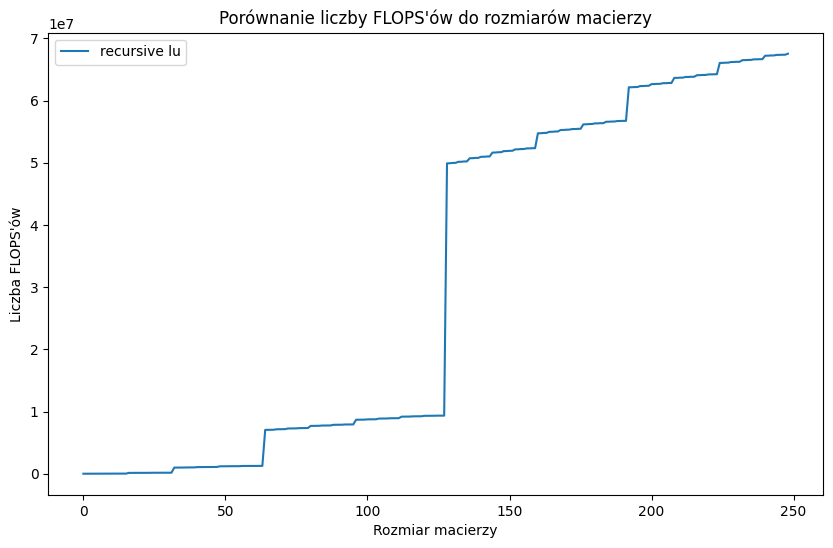
\includegraphics[width=0.99\textwidth]{inverse_flops.png}
  \caption{Wykres sumarycznej liczba FLOPS'ów dla rekurencyjnego odwracania macierzy}
\end{figure}

\noindent
Finalnie sporzadziliśmy wykres czasu działania od rozmiaru macierzy.

\begin{figure}[H]
  \centering
    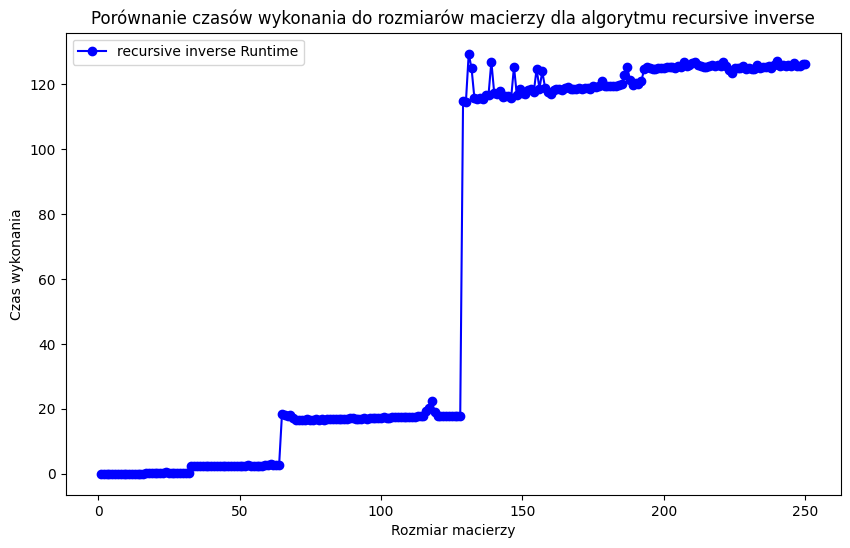
\includegraphics[width=0.99\textwidth]{inverse_time.png}
  \caption{Wykres czasu wykonania w zalezności od rozmiaru macierzy dla rekurencyjnego odwracania macierzy}
\end{figure}

\subsection{Rekurencyjna LU faktoryzacja}

Po przeprowadzeniu pomiarów sporządziliśmy tabelę zawierającą liczby FLOPS'ów dla wybranych rozmiarów macierzy.

\begin{table}[!ht]
    \centering
    \begin{tabular}{|l|l|l|l|}
    \hline
        Rozmiar macierzy & Mnożenie & Dodawanie & Odejmowanie \\ \hline
        2 & 5 & 0 & 1 \\ \hline
        50 & 207393 & 663721 & 319537 \\ \hline
        100 & 1455057 & 4890885 & 2351520 \\ \hline
        150 & 9653187 & 28923656 & 13298213 \\ \hline
        200 & 10198893 & 35230231 & 16940640 \\ \hline
        250 & 10359973 & 38275181 & 18897262 \\ \hline
    \end{tabular}
\end{table}

\noindent
Poniżej znajduje się wykres prezentujący sumę operacji zmiennoprecinkowych
dla rozmiarów macierzy od 1 do 250.

\begin{figure}[H]
  \centering
    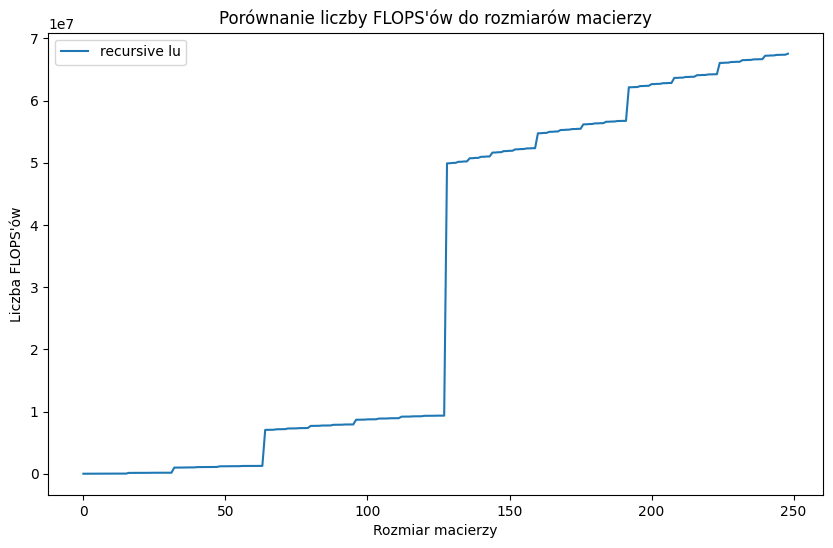
\includegraphics[width=0.99\textwidth]{lu_flops.png}
  \caption{Wykres sumarycznej liczba FLOPS'ów dla rekurencyjnej LU faktoryzacji}
\end{figure}

\noindent
Na końcu sporzadziliśmy wykres czasu działania od rozmiaru macierzy.

\begin{figure}[H]
  \centering
    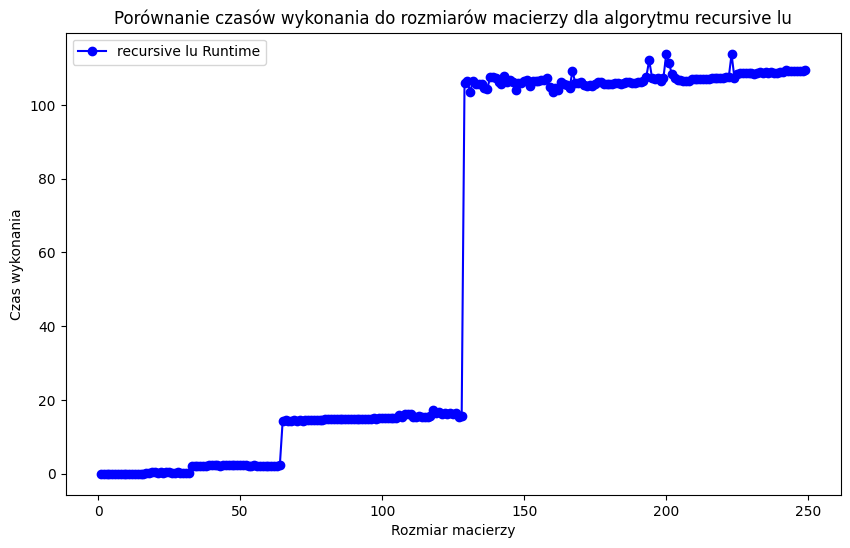
\includegraphics[width=0.99\textwidth]{lu_time.png}
  \caption{Wykres czasu wykonania w zalezności od rozmiaru macierzy dla rekurencyjnej LU faktoryzacji}
\end{figure}

\subsection{Rekurencyjna eliminacja Gaussa}

Pnownie po przeprowadzeniu pomiarów sporządziliśmy tabelę zawierającą liczby FLOPS'ów dla wybranych rozmiarów macierzy.

\begin{table}[!ht]
    \centering
    \begin{tabular}{|l|l|l|l|}
    \hline
        Rozmiar macierzy & Mnożenie & Dodawanie & Odejmowanie \\ \hline
        2 & 8 & 0 & 1 \\ \hline
        50 & 275250 & 880253 & 423244 \\ \hline
        100 & 1924281 & 6464124 & 3105401 \\ \hline
        150 & 12725180 & 38129527 & 17525345 \\ \hline
        200 & 13464465 & 46480441 & 22338954 \\ \hline
        250 & 13698407 & 50537636 & 24936894 \\ \hline
    \end{tabular}
\end{table}

\noindent
Poniżej znajduje się wykres prezentujący sumę operacji zmiennoprecinkowych
dla rozmiarów macierzy od 1 do 250.

\begin{figure}[H]
  \centering
    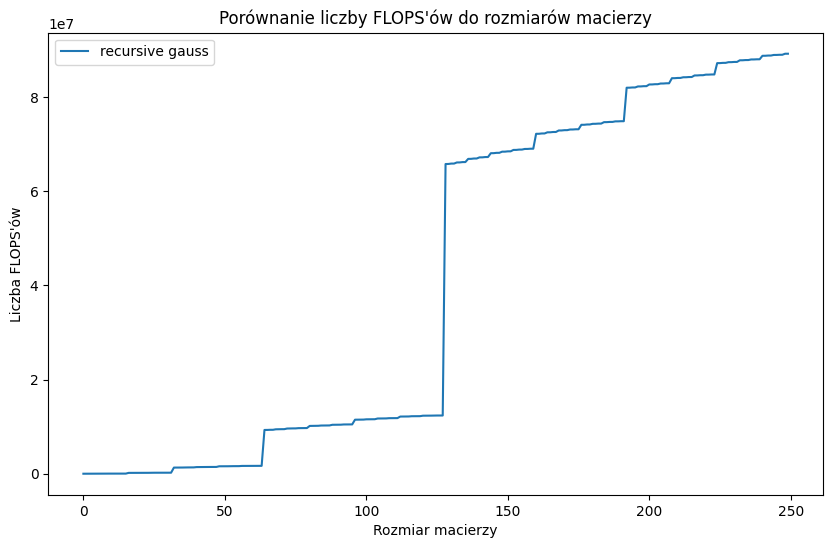
\includegraphics[width=0.99\textwidth]{gauss_flops.png}
  \caption{Wykres sumarycznej liczba FLOPS'ów dla rekurencyjnej eliminacji Gaussa}
\end{figure}

\noindent
Finalnie sporzadziliśmy wykres czasu działania od rozmiaru macierzy.

\begin{figure}[H]
  \centering
    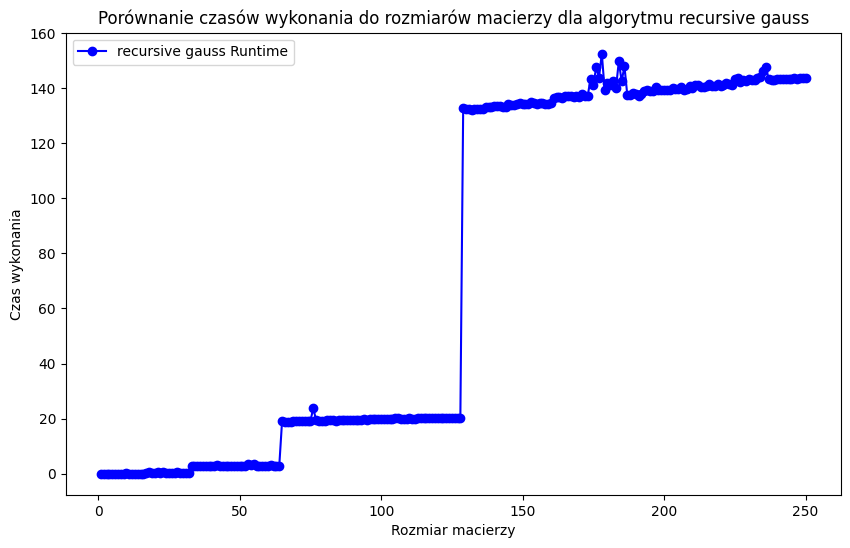
\includegraphics[width=0.99\textwidth]{gauss_time.png}
  \caption{Wykres czasu wykonania w zalezności od rozmiaru macierzy dla rekurencyjnej eliminacji Gaussa}
\end{figure}

\subsection{Rekurencyjne liczenie wyznacznika macierzy}

Tak jak poprzednio sporządziliśmy tabelę zawierającą liczby FLOPS'ów dla wybranych rozmiarów macierzy.

\begin{table}[!ht]
    \centering
    \begin{tabular}{|l|l|l|l|}
    \hline
        Rozmiar macierzy & Mnożenie & Dodawanie & Odejmowanie  \\ \hline
        2 & 7 & 0 & 1  \\ \hline
        50 & 207443 & 663721 & 319537  \\ \hline
        100 & 1455157 & 4890885 & 2351520  \\ \hline
        150 & 9653337 & 28923656 & 13298213  \\ \hline
        200 & 10199093 & 35230231 & 16940640  \\ \hline
        250 & 10360223 & 38275181 & 18897262 \\ \hline
    \end{tabular}
\end{table}

\noindent
Poniżej znajduje się wykres prezentujący sumę operacji zmiennoprecinkowych
dla rozmiarów macierzy od 1 do 250.

\begin{figure}[H]
  \centering
    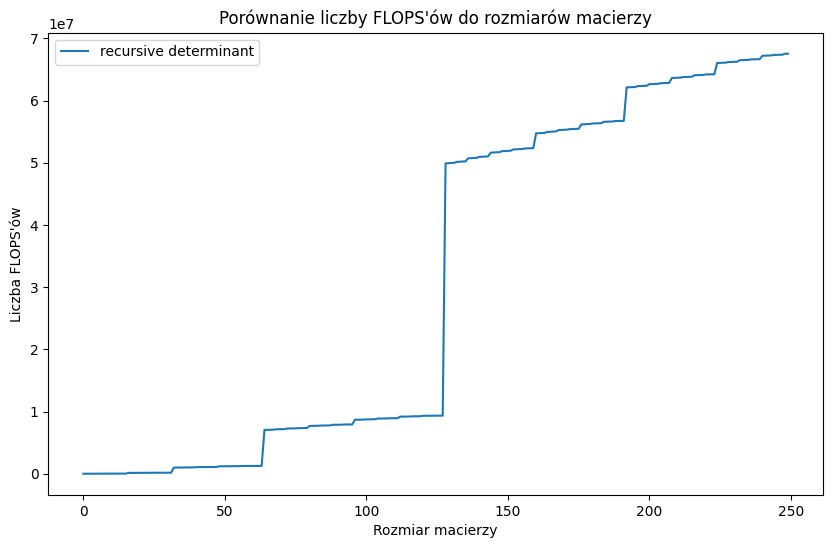
\includegraphics[width=0.99\textwidth]{images/determinant_flops.png}
  \caption{Wykres sumarycznej liczba FLOPS'ów dla rekurencyjnego liczenia wyznacznika}
\end{figure}

\noindent
Finalnie sporzadziliśmy wykres czasu działania od rozmiaru macierzy.

\begin{figure}[H]
  \centering
    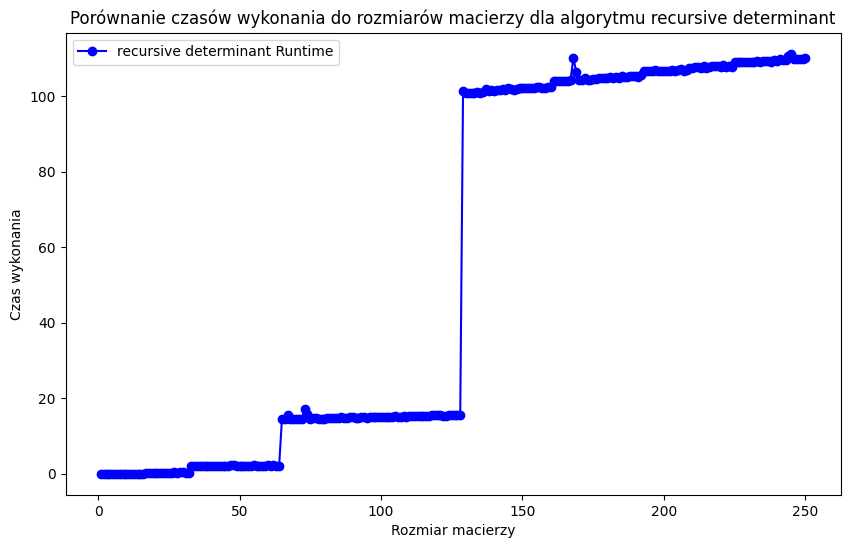
\includegraphics[width=0.99\textwidth]{images/determinant_time.png}
  \caption{Wykres czasu wykonania w zalezności od rozmiaru macierzy dla rekurencyjnego liczenia wyznacznika}
\end{figure}

\section{Porównanie liczby operacji zmiennoprzecikowych i czasów wykonania}

Zdecydowaliśmy się również sporządzić wykresy obrazujące jak ma się liczba operacji zmiennoprzecinkowych między sobą dla rozważanych algorytmów i to samo zrobić dla czasów wykonania.

\bigbreak

\noindent
Porównanie liczby operacji zmiennoprzecinkowych:

\begin{figure}[H]
  \centering
    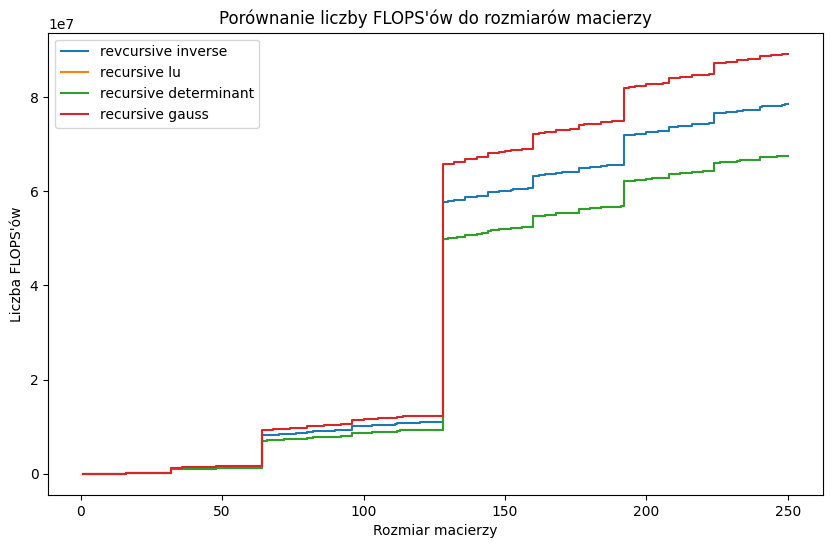
\includegraphics[width=0.99\textwidth]{flops_comparison.png}
  \caption{Porównanie sumarycznej liczby FLOPS'ów dla wszyskich rozważanych algorytmów}
\end{figure}

\bigbreak

\noindent
Porównanie czasów działania:

\begin{figure}[H]
  \centering
    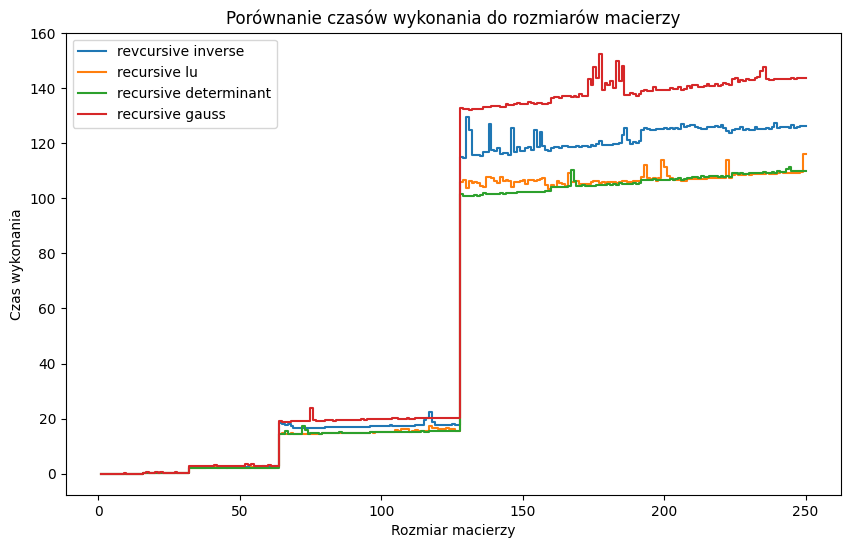
\includegraphics[width=0.99\textwidth]{time_comparison.png}
  \caption{Porównanie czasów działania dla wszyskich rozważanych algorytmów}
\end{figure}

\section{Oszacowanie złożoności obliczeniowej}

\noindent
Z powodu wykorzystania algorytmu Strassena w algorytmach rekurencyjnych spodziewaliśmy się otrzymać złożoność obliczeniową w okolicach \(n^{2.81}\). Aby potwierdzić nasze przypuszczenia postanowiliśy dopasować krzywą tej złożoności do otrzymanych wykresów czasów wykonania.

\begin{figure}[H]
    \centering
    \begin{minipage}{0.45\textwidth}
        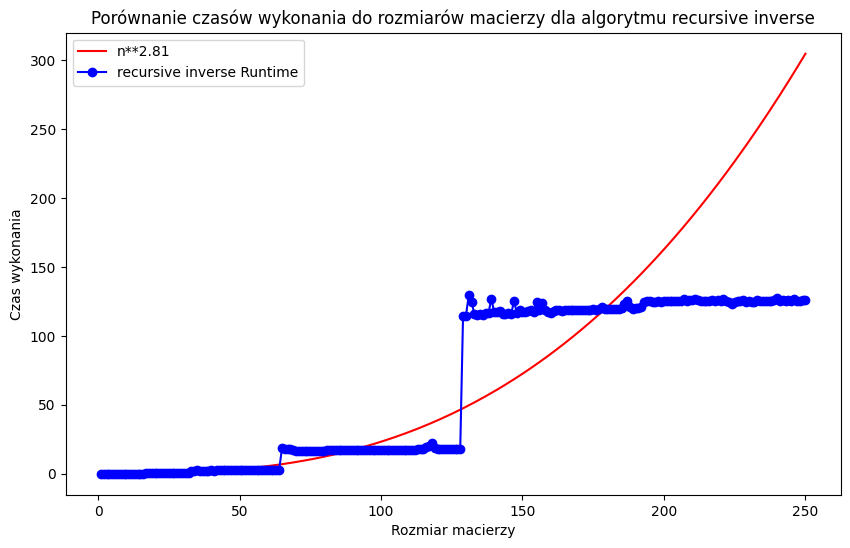
\includegraphics[width=\linewidth]{images/inverse_curve.png}
        \caption{Dopasowanie krzywej złożoności do wykresu czasu działania rekurencyjnego odwracania macierzy}
    \end{minipage}%
    \hfill
    \begin{minipage}{0.45\textwidth}
        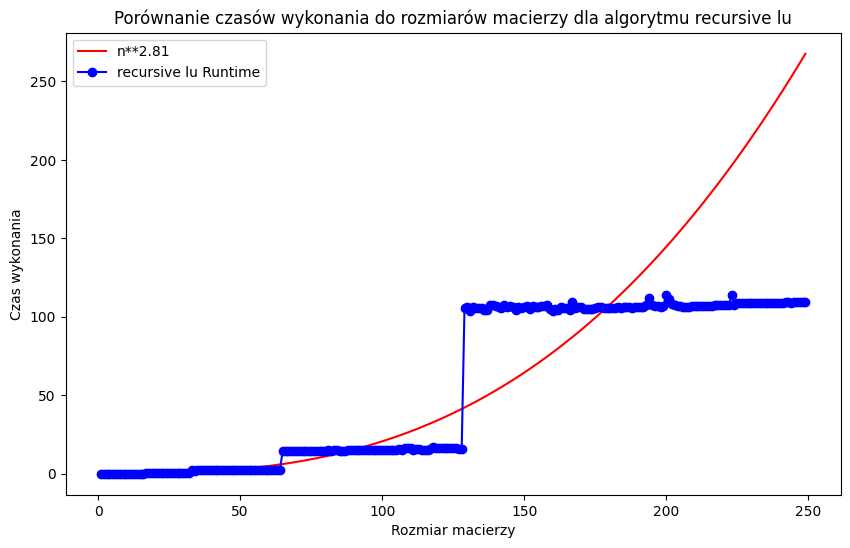
\includegraphics[width=\linewidth]{images/lu_curve.png}
        \caption{Dopasowanie krzywej złożoności do wykresu czasu działania rekurencyjnej LU faktoryzacji}
    \end{minipage}

    \vspace{0.5cm} % odstęp między wierszami

    \begin{minipage}{0.45\textwidth}
        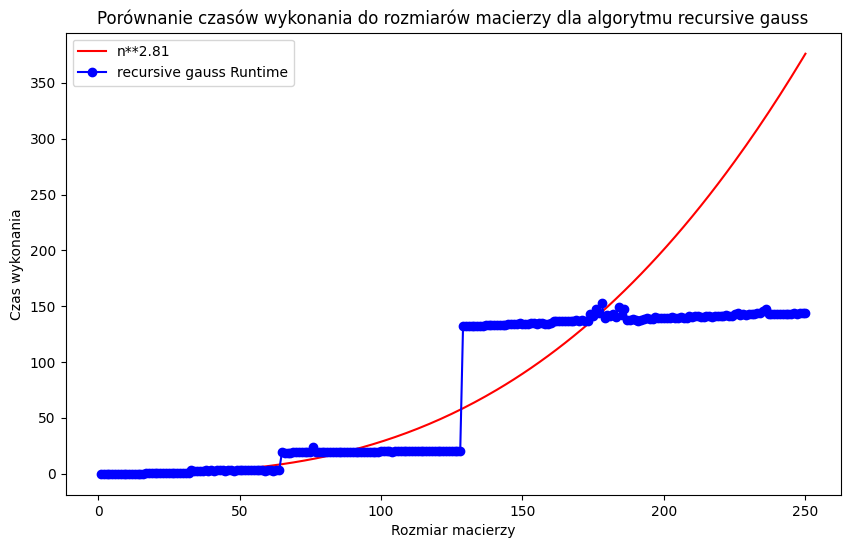
\includegraphics[width=\linewidth]{images/gauss_curve.png}
        \caption{Dopasowanie krzywej złożoności do wykresu czasu działania rekurencyjnej eliminacji Gaussa}
    \end{minipage}%
    \hfill
    \begin{minipage}{0.45\textwidth}
        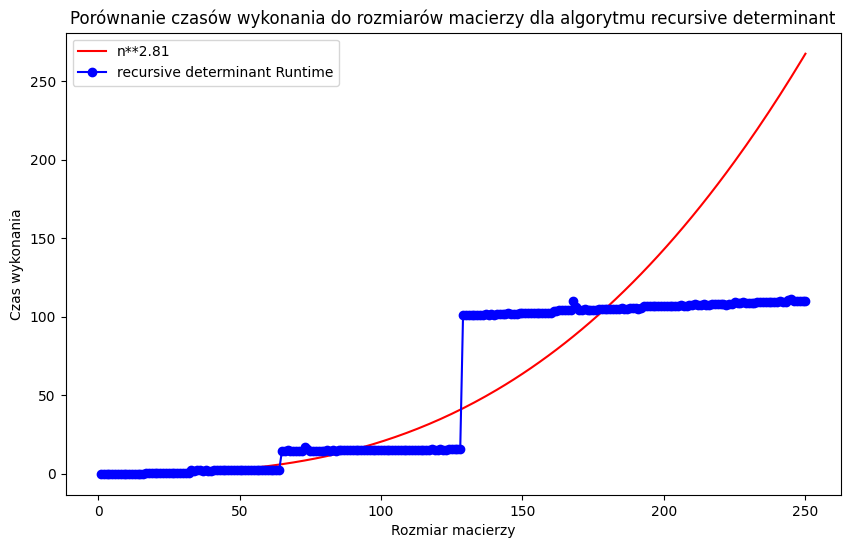
\includegraphics[width=\linewidth]{images/determinant_curve.png}
        \caption{Dopasowanie krzywej złożoności do wykresu czasu działania rekurencyjnego liczenia wyznacznika macierzy}
    \end{minipage}
\end{figure}

\noindent
Jak widać na powyższych wykresach nasze przypuszczenia się potwierdziły.

\section{Porównanie wyników z Octave}

\subsection{Rekurencyjne odwracanie macierzy}

Przeprowadziliśmy testy dla macierzy:

\[
A = \begin{bmatrix}
1.12 & 6.31 & 3.52 & 5.31 & 3.23 \\
2.43 & 5.23 & 7.43 & 6.54 & 2.22 \\
0.76 & 4.98 & 7.86 & 4.00 & 7.43 \\
9.99 & 4.33 & 5.44 & 3.45 & 2.45 \\
6.43 & 5.44 & 3.23 & 1.23 & 2.67
\end{bmatrix}
\]

\noindent
Otrzymane wyniki to:

\begin{figure}[H]
  \begin{minipage}[b]{0.49\textwidth}
    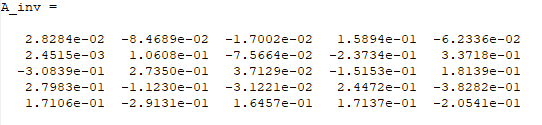
\includegraphics[width=\textwidth]{images/octave_comparison_inversion_octave.png}
    \caption{Wyniki dla odwracania macierzy otrzymane z wykorzystaniem Octave}
  \end{minipage}
  \hfill
  \begin{minipage}[b]{0.49\textwidth}
    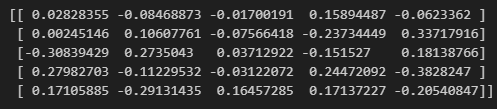
\includegraphics[width=\textwidth]{images/octave_comparison_inversion_own.png}
    \caption{Wyniki dla odwracania macierzy otrzymane z wykorzystaniem własnej implementacji}
  \end{minipage}
\end{figure}

\bigbreak

\noindent
Jak widać wyniki są takie same.

\subsection{Rekurencyjna LU faktoryzacja}

Ponownie wykorzystaliśmy macierz z poprzedniego podpunktu. Otrzymane wyniki:

\begin{figure}[H]
  \begin{minipage}[b]{0.49\textwidth}
    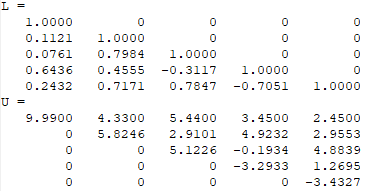
\includegraphics[width=\textwidth]{images/octave_comparison_lu_octave.png}
    \caption{Wyniki dla lu faktoryzacji macierzy otrzymane z wykorzystaniem Octave}
  \end{minipage}
  \hfill
  \begin{minipage}[b]{0.49\textwidth}
    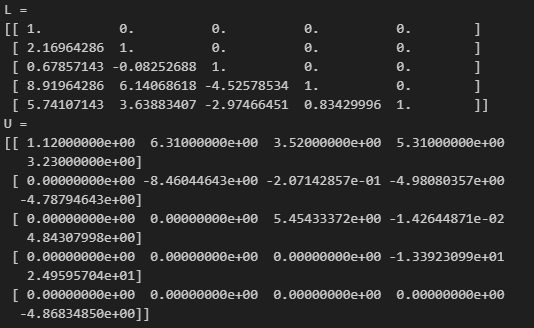
\includegraphics[width=\textwidth]{images/octave_comparison_lu_own.png}
    \caption{Wyniki dla lu faktoryzacji macierzy otrzymane z wykorzystaniem własnej implementacji}
  \end{minipage}
\end{figure}

\noindent
Wyniki się nie zgadzają.

\subsection{Rekurencyjna eliminacja Gaussa}

Testy zostały przeprowadzone dla tej samej macierzy A oraz wektora b:

\[\mathbf{b} = \begin{bmatrix} 1.23 \\ 2.12 \\ 7.54 \\ 8.55 \\ 3.45 \end{bmatrix}\]

\noindent
Oto otrzymane wyniki:

\begin{figure}[H]
  \begin{minipage}[b]{0.49\textwidth}
    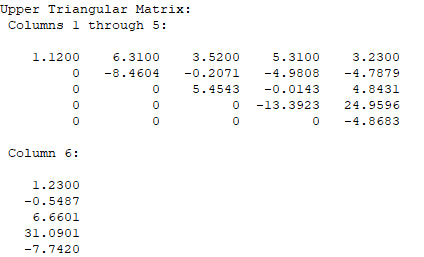
\includegraphics[width=\textwidth]{images/octave_comparison_gauss_octave.png}
    \caption{Wyniki dla eliminacji gaussa otrzymane z wykorzystaniem Octave}
  \end{minipage}
  \hfill
  \begin{minipage}[b]{0.49\textwidth}
    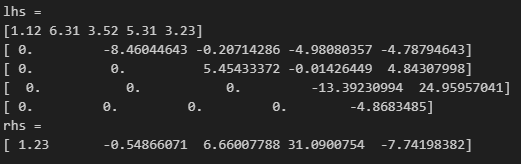
\includegraphics[width=\textwidth]{images/octave_comparison_gauss_own.png}
    \caption{Wyniki dla eliminacji gaussa  otrzymane z wykorzystaniem własnej implementacji}
  \end{minipage}
\end{figure}

Jak widać na powyższych rysunkach wyniki się zgadzają

\subsection{Rekurencyjne liczenie wyznacznika}

Test został przeprowadzony na macierzy A opisanej powyżej.

\noindent
Oto otrzymane wyniki:

\begin{figure}[H]
  \begin{minipage}[b]{0.49\textwidth}
    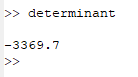
\includegraphics[width=\textwidth]{images/octave_comparison_determinant_octave.png}
    \caption{Wyniki dla rekurencyjnego liczenia wyznacznika otrzymane z wykorzystaniem Octave}
  \end{minipage}
  \hfill
  \begin{minipage}[b]{0.49\textwidth}
    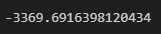
\includegraphics[width=\textwidth]{images/octave_comparison_determinant_own.png}
    \caption{Wyniki dla rekurencyjnego liczenia wyznacznika z wykorzystaniem własnej implementacji}
  \end{minipage}
\end{figure}

\noindent
Wynik uzyskany z Octave został zaokrąglony, ale i tak można stwierdzić, że nasza metoda jest poprawna.

\section{Wnioski}

\begin{itemize}
    \item Algorytm Strassena okazuje się bardzo przydatny przy implementacji opisanych algorytmów
    \item Octave jest dość intuicyjne i posiada sporo wbudowanych funkcji, które pozwalają wykonywać podstawowe operacje macierzowe.
    \item Podejście rekurencyjne sprawia, że implementacja rozważanych algorytmów jest dość intuicyjna i prosta.
    \item Mimo złożoności rzędu \(n^{2.81}\) algorytmy wykonują się BARDZO długo dla macierzy o rozmiarach liczonych w setkach.
    \item Po porównaniu wyników naszych algorytmów z Octave, przekonaliśmy się, że nasza implementacja jest poprawna.
\end{itemize}

\section{Źródła}

\begin{enumerate}
    \item Wykład z kursu "Algorytmy Macierzowe"
    \item Dokumentacja Octave - https://docs.octave.org/latest/
\end{enumerate}


\end{document}
